%%%%%%%%%%%%%%%%%%%%% RJT TeX Template %%%%%%%%%%%%%%%%%%%%%
\documentclass[twoside,12pt,a4paper]{article}

%%%% BHAM PREAMBLE - SET THIS FIRST! %%%%
\newcommand{\bhamstudentname}{Zhangda Xu}
\newcommand{\bhamthesistitle}{Play Curling with Deep Reinforcement Learning}
\newcommand{\bhamfronttitle}{Play Curling with \\ Deep Reinforcement Learning}
\newcommand{\bhamschool}{School of Computer Science}
\newcommand{\bhamcollege}{Engineering and Physical Sciences}
\newcommand{\bhamdegree}{Advanced Computer Science}
\newcommand{\bhamid}{2088192}
\newcommand{\bhamsupervisor}{Mohan Sridharan}
\newcommand{\bhamyear}{2020}
%%%%           %%%%


\usepackage[hyphens]{url}
\usepackage[breaklinks]{hyperref}
\usepackage{fancyhdr}
\usepackage[sort]{natbib}
\usepackage{comment}
\usepackage{dirtree}
\usepackage{longtable}
\usepackage{algorithm}
\usepackage{algorithmic}

\renewcommand{\algorithmiccomment}[1]{#1}

\pagestyle{fancy}
\renewcommand{\sectionmark}[1]{\markboth{#1}{}}

\lfoot{\bhamstudentname}
\cfoot{}
\rfoot{}
\fancyhfoffset[L]{0cm}
\newcommand{\HRule}{\rule{\linewidth}{0.5mm}}
\renewcommand{\headrulewidth}{0pt}
\newcommand{\tab}{\hspace*{1.25em}}
\newcommand{\minitab}{\hspace*{0.25em}}

\usepackage{perpage}
\MakePerPage{footnote}
\renewcommand*{\thefootnote}{\fnsymbol{footnote}}

\lhead{}\chead{}\rhead{}
\setlength{\headheight}{28pt}
\setlength{\headsep}{6pt}
\pdfoutput=1
\usepackage[left=2.55cm,right=1.6cm,top=1.8cm,bottom=1.8cm]{geometry}
\usepackage{titling}
\setlength{\droptitle}{-2.75cm}
\usepackage{titlesec}
\titleformat*{\section}{\normalsize	\bfseries}
\titleformat*{\subsection}{\small \bfseries}
\titleformat*{\subsubsection}{\footnotesize \bfseries}

\titlespacing*{\section} {0pt}{3ex plus 1ex minus .2ex}{2ex plus .2ex}
\titlespacing*{\subsection} {0pt}{2.25ex plus 1ex minus .2ex}{0.75ex plus .2ex}
\titlespacing*{\subsubsection}{0pt}{2.ex plus 1ex minus .2ex}{0.5ex plus .2ex}

\setlength{\intextsep}{0pt}

\usepackage[pdftex]{graphicx}
\usepackage{enumitem}
\usepackage{pdfpages}
\usepackage{lastpage}
\usepackage{amsmath}
\usepackage{amsfonts}
\usepackage{amssymb}

\usepackage{epstopdf}

\usepackage{listings}
\lstset{
 basicstyle=\ttfamily,
  columns=fullflexible,
  keepspaces=true,
breaklines=true
}

\newcommand{\todo}[1]{\textcolor{red}{TODO: #1}\PackageWarning{TODO:}{TODO found: #1!}}

\DeclareGraphicsExtensions{.jpg}

%%%%%%%%%%%%%%%%%%%%%  END of TEMPLATE %%%%%%%%%%%%%%%%%%%%%


\title{MSc. Project\\\bhamthesistitle}
\author{\textsf{\bhamstudentname }}

\date{}
\begin{document}

\pagenumbering{gobble}
\begin{titlepage}
\begin{center}
\begin{minipage}{6in}
  \centering
  \raisebox{-0.5\height}{
\includegraphics[width=1.25in]{crest}}
  \hspace*{.2in}
  \raisebox{-0.5\height}{
\includegraphics[height=0.9375in]{uni}}
  \end{minipage}
  \\ [1.0cm]
\textsc{{\LARGE \bhamschool\\}College of \bhamcollege}\\[3.5cm]

\textsc{\Large MSc. Project}\\[0.5cm]

% Title
\HRule \\[0.4cm]
\begin{center}\Huge
\bhamfronttitle
\end{center}
\HRule \\[1.5cm]

\begin{center}
Submitted for the degree of MSc. \\ \textbf{{\large \bhamdegree}}\\
\vspace{1.5cm}
{\Large \textbf{\bhamstudentname}}\\
Student ID: \bhamid\\
\vspace{1.5cm}
{\Large Supervisor: \bhamsupervisor}
\end{center}
\vfill

% Bottom of the page
{\large September \bhamyear}

\end{center}
\end{titlepage}

% Table of Contents
\clearpage
\maketitle
\vspace{-5.5em}
\begingroup
\fontsize{9pt}{11pt}\selectfont
\tableofcontents
\endgroup
\clearpage
\phantomsection

\section{Abstract}
% Paragraph
Placeholder.

\section{Introduction}
% Citation
hello! \citep{RailExecutive14a}

\section{Theory}
% Math
$ d = p * g $
\[ dql = - \frac{1}{2} \log n \]

\section{Method}
% Image
\begin{center}
    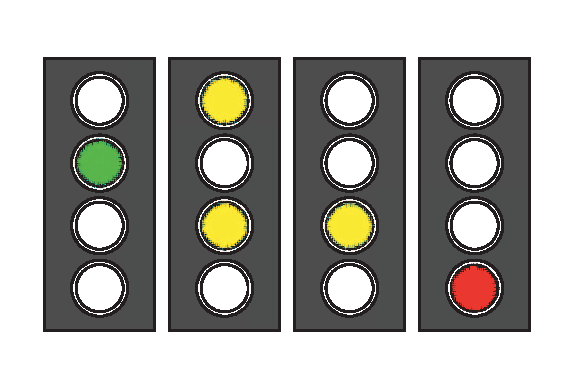
\includegraphics[scale=.25]{Signals-eps-converted-to.pdf}\\
    Figure 4.1: \textit{Reference Driver Machine Interface \citep{RailExecutive14a}}
\end{center}

\section{Implementation}
% Algorithm
\begin{algorithm}[H]
    \floatname{algorithm}{EuroRadio Protocol}
    \renewcommand{\thealgorithm}{}
    \caption{Steps that an ERTMS Entity would undertake to establish a connection}
    T: Train, R: Radio Block Centre, $K_{MAC}$: Train Key, $KS_{MAC}$: Session Key
    \label{EuroRadio Protocol}
    \begin{algorithmic}[1]
        \STATE $T\rightarrow{R}$ : \{\texttt{ETY},\texttt{MTI}$\gets$AU1, \texttt{DF}$\gets$0, Sender ETCS ID, Safety Feature, R$_T$\}.
        \texttt{DF}, Padding))\}
    \end{algorithmic}
\end{algorithm}

\section{Experiment}
% Tabular
\begin{center}
    \begin{longtable}{|c|c|}

        \hline \multicolumn{1}{|c|}{\textbf{Threat}} & \multicolumn{1}{c|}{\textbf{EuroRadio}} \\ \hline \hline
        \endfirsthead

        \multicolumn{2}{c}%
        {{\bfseries Threat/Defence Matrix -- continued from previous page}} \\
        \hline \multicolumn{1}{|c|}{\textbf{Threat}} & \multicolumn{1}{c|}{\textbf{EuroRadio}} \\ \hline \hline
        \endhead

        \multicolumn{2}{|r|}{{Continued on next page}} \\ \hline
        \endfoot

        \hline \hline
        \endlastfoot

        Repetition & $\times$ \\ \hline
        Deletion & $\times$ \\ \hline
        Insertion & \checkmark \\ \hline
        Re-sequencing & $\times$ \\ \hline
        Corruption & \checkmark \\ \hline
        Delay & $\times$ \\ \hline
        Masquerade & \checkmark \\ \hline

    \end{longtable}
\end{center}

\section{Discussion}
% List
\begin{itemize}[nolistsep]
    \item 3DES -- Triple DES
    \item 3G -- Third Generation
    \item AES -- Advanced Encryption Standard
    \item ALE -- Adaptation Layer Entity
\end{itemize}


\section{Conclusion}
# Curling with Deep Reinforcement Learning



## Abstract .2k

The problem that this project aims to solve is one of the task completion for intelligent agents in a tabletop environment. In the context of a practical setting, the agent learns to play curling on the surface with an improved control policy when observing the environment. Works in the project is intended to explore the application of various theoretical approaches in the field of reinforcement learning. The method proposed here takes in the rendered observation of environment directly as pixel input, and learn through deep neural networks end-to-end with returned policies. To simulate physics and conduct the experiments, we uses PyBullet engine as an simulated environment with models of objects. Curling game play involves continuous control over the agent. The algorithm used for the task needs to update agent's deterministic policy for the given scenarios to improve convergence. During the training process, the agent is enabled to learn from past experiences of play to update current policies using a memory buffer. We propose a model with an *actor-critic* architecture, integrating the deep deterministic policy gradient method with a memory layer. We show that our model can be successfully applied on the curling game play task and other classic reinforcement learning tasks. Comparing with existing state-of-the-art methods, the result indicates the improvement in stability and generalisation due to the proposed modification.



## Introduction 1k

The problem of agent control often involves the interaction with the environment. The goal here is to make good sequential decisions of actions given arbitrary situation of the environment. It is natural to consider both the agent and the environment where it locates when control problem is to be solved. However, from the agent's perspective, the mechanics behind the world is often not known or incomplete, which makes it inapplicable for planning and prediction tasks. Instead, the agent needs a *try-and-error* approach to learn from interactions with the environment, improving its own knowledge of the environment and how to choose actions next time. It is proved that agent is guaranteed to improve the control through learning.

The problem of learning is one of the most studied fields in machine learning. By definition, learning for an intelligence refers to the process of putting together a sequence of thoughts and actions, assisted by perception and observation of the environment. Artificial learning behaviour is similar to that of animal's. Generally, we have three paradigms to solve the learning problem: supervised learning, unsupervised learning and reinforcement learning. In supervised learning, the learner is trained with pre-labelled data to predict the result or labels given the raw input. We judge the performance of learner's predictions by comparing it with given results of known samples, where the feedback is often in the form of an optimisation term, or a similarity ratio. Unsupervised learning requires no prior knowledge of the labels of data, but only exploit the internal relationship between the data. On the whole, both approaches assume the data collected for prediction tasks to be identically and independently distributed. When is faced with the control task, both paradigms cannot fit properly for the purpose of sequential decision making.

Reinforcement learning provides a better method to model the agent control task. A reinforcement learning world splits off the agent from its surrounding environment that out of the agent's control. The interactions between agent and environment are considered in a sequence of time steps. At every time step, the environment emits a scalar reward as the feedback, but no supervisor is needed. The reward signal is the goal of a reinforcement learning problem, which is analogous to positive or negative experiences of the agent. Thus the process of control is formulated as consecutive maximisation of the total reward. In addition, reinforcement learning enables the usage of correlated data obtained at different time, whose distribution is not invariant through learning.

In this project, we propose to study the control of curling game play. Curling is a sports game where players in both teams slide stones on a sheet of icy surface toward a target area, which is segmented into four concentric circles. The smaller the circle is, the more the stones in it will score at the end of a game. The goal of the competition is to beat the other team in total scores on the ice. Each team takes turns to complete a round of throwing, with one player responsible for the throw and others responsible for sweeping on the ice to control the path of stone. There are various strategies for curling game play. Sometimes the key to victory lies not only in the precision of throwing, but rather to harass the positioning of opponent's stones. It is reasonable to pave the way for a better opportunity in the next round as well.

The task of curling considered in the project is simplified to be a single round throw without assistant sweeping. By isolating decision making in consecutive rounds, we ignore the higher-level competitive game play consideration at this stage, focusing on the optimisation of throw control only. The problem of controlling the agent thus becomes: to search for the best initial velocity and angle of throw given the current positioning of friendly and opposite stones on the court, i.e. the best policy to play this round. Note that the actions to choose will be on a continuous space, if we look for a fine control on the agent.

Recent advances in deep neural network makes it possible to learn the control policy directly from sensory inputs, such as high-dimensional visual data. Deep multi-layer perceptrons are capable of extracting high-level representations of the original data, which make hand-picked features obsolete. In order to learn end-to-end, we need to make use of the agent's observations of the environment to discover the optimal policy. However, reinforcement learning takes the try-and-error approach, which may incur unrecoverable repercussions in physical experiments. On the other hand, the captured vision or speech is often too noisy to use for learning task. We avoid these obstacles by using a simulated environment in PyBullet, where all the physics are handled with by the engine and visuals are rendered as the final output. Most parts of the software will be implemented in this ecosystem.

<Need editing>

This project is intended to solve the problem of curling game play using deep reinforcement learning. This report first establishes the theoretical ground of using such technique, and concludes the previous related work for comprehensive insights. Then, we formulate the state-of-the-art solution for similar problems and show that practical improvements are required for this specific task. The implementation of the whole architecture is discussed in detail. We later present the experiments of the proposed algorithms and compare it with existing variants. We finally evaluate the results in depth and validate the proposed methods. The software developed so far in this project is able to visualise the process of training and simulations. The performance of the algorithm is proved to be stable and outperform the average human player.



## Theory 2k

In this section, we introduce the preliminaries needed to formulate both the problem and solutions in reinforcement learning.



#### 2.1 Reinforcement Learning

In a reinforcement learning paradigm, we consider the control task of the cue stone interacting with the environment of a curling court. The agent can be thought as a self-controllable intelligent stone or an external robotic arm that exerts an initial push on it. In either case, at each time step $t$, the agent selects an action from the space of all legit actions $a_t \in\mathcal A$, given the current state $s_t \in \mathcal S$. Since the internal state of the environment is not known to the agent, we treat the observation of the simulated environment $\mathcal O$, which is rendered from a stationary point of view, as a full representation of the state. As a response to the agent, the emulator then emits a reward $R_t$ and the new state $s_{t+1}$ after receiving the action-state pair. A basic representation of reinforcement learning can be given as a tuple:
$$
\left\langle \mathcal {S,A, R} \right\rangle
$$
The reward $r_t$ is a feedback signal which indicates how well the agent is doing at time step $t$. Although it is arbitrary to design the reward signals, the reward hypothesis states that all goals of the agent should be described by the maximisation of expected cumulative reward. The instant reward in the current state $R_t$ for an action $a_t$ alone is not a complete feedback of how good the action is, because it ignores its potential effects on the environment and the following states. We instead define the return $G_t$ of an episodic task as the total discounted reward starting from time step $t$:
$$
G_t = R_{t+1} + \gamma R_{t+2}, +\gamma^2 R_{t+3}+... = \sum_{k=0}^\infty\gamma^kR_{t+k+1}
$$
Here $\gamma$ is a discount parameter applied to every consequent reward in the future, where each component represents the present value of future rewards. We use the discounted version of the total reward for several reasons. First, it correctly models the uncertainty about the future in the process. It also incorporates the common preference of immediate reward over delayed ones. Lastly, it can avoid infinite returns for cyclic process.



#### 2.2 Markov Decision Process

We next formulate the environment of reinforcement learning with Markov decision process. A state is considered Markov if and only if the current state captures all relevant information from the history. It means that given the current state, to predict the future states, all the previous history can be thrown away. In the form of a conditional probability, the next state is independent of past history:
$$
\mathbb P[S_{t+1}|S_t]=\mathbb P[S_{t+1}|S_1,...,S_t]
$$
A Markov decision process is where all the states are Markov. Most reinforcement learning problems can be simplified as MDPs so that there is no need for deduction of what happened in the past. In a tabular representation, the probability of each possible successor state is described by the state transition matrix:
$$
\mathcal P_{ss'}^a=\mathbb P[S_{t+1}=s'|S_t=s, A_t=a]
$$
The goal in MDP is to find the best behaviours for the agent in the face of different states. We define the policy $\pi$ as a mapping of actions given states:
$$
\pi(a|s) = \mathbb P[A_t=a|S_t=s]
$$
Since the state is a sufficient statistic for the environment, the policy is a stationary distribution of behaviours given the state: $A_t \sim \pi(\cdot|S_t)$. We can use the policy to rewrite the reward function following a fixed policy in a form of expectation:
$$
\mathcal R_s^\pi = \sum_{a\in \mathcal A}\pi(a|s)\mathcal R_s^a
$$



#### 2.3 Value Function

Recall that the purpose of an agent in reinforcement learning is to maximise the expected value of the total reward. We can formulate the state-value function of a state $s$ under a policy $\pi$ as the expected return starting from the current state, following policy $\pi$:
$$
v_\pi(s) = \mathbb E_\pi[G_t|S_t=t]
$$
The action-value further incorporates the value of actions into the value of current state, which is often preferred in reinforcement learning problems because it is solely dependent on the environment. Similarly, it describes the value of taking action $a$ given a state $s$, following a policy $\pi$ in next steps:
$$
q_\pi(s,a) = \mathbb E_\pi[G_t|S_t = t, A_t = a]
$$
Due to the recursive property of the return, we can decompose the return at time-step $t$ into an immediate reward and the expected value of successor states. This one-step look-ahead can be used as the update rule of action-values, which enables the recursive evaluation of current policy. This is known as the Bellman equation:
$$
q_\pi(s_t,a_t) = \mathbb E_\pi[R_{t+1} + \gamma\mathbb E_\pi [q_\pi(s_{t+1}, a_{t+1})]]
$$
Here the expectation of the action-value given the current state-action pair is the backup of the complete transition, where every successor state is used in a sweep recursively until the end of episode. Although the Bellman update makes use of dynamic programming to reduce space complexity, it still causes huge cost of unnecessary memory. This requires a full backup of the entire process, including the knowledge of complete transitions and rewards. In practice, it is hardly known to the agent. Instead, the agent needs to learn from episodes of its experience.

Temporal-difference learning is a policy evaluation method that can learn from incomplete sequences without the model of Markov decision process. It explores the Markov property of states using bootstrapping and sampling simultaneously. Like the Monte Carlo method, TD learning uses sampled episodes instead of an exhaustive search to approximate the expectation term in the equation, in which a full process is explored until the terminal state. TD learning is also bootstrapping, which enables it to learn from incomplete episodes even without the final outcome. The main idea is to update the functions towards another belief of the state. Consider the simplest variant TD(0), the algorithm updates the value function $v(s_t)$ online towards an estimated return at the next time-step:
$$
V(S_t)\larr V(S_t)+\alpha(R_{t+1}+\gamma V(S_{t+1})-V(S_t))
$$
Here $R_{t+1}+\gamma V(S_{t+1})$ is the TD target, $\alpha$ is the step parameter, which ensures continuous update towards the TD target. It can be proved that TD(0) converges to solution of maximum likelihood estimate of Markov model that best fit the data. Temporal-difference learning introduces bias to the estimate but lowers the total variance, because the TD target only depends on one state transition and reward. It is also a much cheaper online update scheme in large scale problems.

It is essential for the agent to improve the policy starting from an initial action. Basically, the agent first needs to evaluate the policy, then updates it iteratively towards the best policy. For any Markov decision process, there always exist one or multiple policy $\pi^*$ that is no worse than any other policies. In general policy iteration processes, the optimal policies are guaranteed to achieve the optimal action-value.



#### 2.4 Policy Gradient

Last section concludes the modelling of a tabular representation of reinforcement learning problems. The whole process is stored as pairs of state and action, where the value of each state is calculated individually. Recent development in sensory data processing requires an efficient architecture for large-scale problem solving. It is common to approximate the functions with parameters, such as linear functions and neural networks, to generalise the problem from known states to unseen states.

Value-based policy iteration improves the policy by acting with respect to the value function. Alternatively, we can directly learn the parameterised policy. In many occasions, value-based policy iteration approaches are unstable to converge to the optimal policy due to the sparse value distribution. The values are not reliable to learn the target policy when stochastic decision making is needed. Moreover, value-based policy improvement cannot effectively model actions in high-dimensional or continuous spaces. Policy-based reinforcement learning promises an optimisation problem over the whole action space. On the other hand, the evaluation of policy is often inefficient and introduces high variance in the process.

Policy gradient algorithms is essentially an optimisation problem searching for a local maximum of a policy objective function. The quality of policy, or the scale of objective, is often related to the rewards in one episode. The gradient describes the direction and the magnitude of most effective ascent of one step update. Policy is updated online using gradient ascent with respect to the parameters. For an approximated policy $\pi_\theta$, with a fixed step size $\alpha$, the updated value of parameters $\Delta \theta$ is given as:
$$
\Delta\theta=\alpha\nabla_\theta J(\theta)
$$
Here $\nabla_\theta J(\theta)$ is the policy graident, which can be calculated analytically. A common practice is to rewrite the original gradient as an expectation of the gradient of the logarithm:
$$
\nabla_\theta J(\theta) = \pi_\theta(s,a)\cdot\nabla_\theta \log\pi_\theta(s,a)
$$
Policy gradient theorem states that for a differentiable policy $\pi_\theta$ approximated by parameters $\theta$ and any policy objective, the policy gradient is given as:
$$
\nabla_\theta J(\theta) = \mathbb E_{\pi_\theta}[\nabla_\theta\log\pi_\theta(s,a)Q^{\pi_\theta}(s,a)]
$$
Here $Q^{\pi_\theta}(s,a)$ is a long-term value for the policy. Policy gradient in the form of an expectation makes it convenient to use stochastic gradient ascent optimisation.

actor-critic



deterministic policy gradient



### 3. method

full information game

action space

observation space

mlp















### 4. Implementation





### 5. Experiment
% Bibliography
\clearpage
\lhead{}\chead{MSc. Project Report :: \nouppercase{\leftmark}}\rhead{}
\phantomsection
\addcontentsline{toc}{section}{References}
\bibliographystyle{agsm}
\bibliography{mybib}

\clearpage

\section{Appendix}
\subsection{Appendix I.}

\end{document}